%!TEX root = iclr2026_conference.tex
% ==== BRIEF §6 HEAD (Results) =========================================================
% [中] 定位：按 §1 的三条发现依次给出证据：粒度改变滚动误差；没有固定请求适合所有发射集；逐预测选择请求可以利用这种差异。
%      每个小节先给结论句，再给数字；与摘要、引言同序、同措辞（"matches ... at a third of its compute"）。
% 卖点：同一个共享潜变量模型在三个 benchmark 上保留长跳跃的精度；最佳请求沿两轴随发射集变化；逐预测选择优于迁移来的固定请求。
%      证据：issue-77-n1-diagnostic-v1、issue-79-clevrer-boundary-v1、issue-84-third-family-v1 的 summary.json（position_mse）；
%            issue-96-tau-ad-within-checkpoint-v1 的 comparisons.csv 与 frequencies.json；issue-74-matched-dynamics-v1/readiness.json；
%            issue-92-lookahead-control-v1 的 hybrid-adaptive-e600 记录（Figure 1a 的轨迹）。
%      手法与边界：区间只作描述；不写显著性；不合并发射集或 benchmark；策略只在 decision-only 想象 rollout 中评估。
% [EN] Role: evidence for the three findings of Section 1, in order: granularity changes rollout error; no fixed request
%      suits every launch set; choosing the request per prediction exploits the variance. Each subsection opens with
%      its claim, then its numbers; wording matches the abstract and introduction.
%      Evidence: summary.json of issue-77 diagnostic, issue-79 and issue-84 (position_mse); issue-96 comparisons.csv and
%      frequencies.json; issue-74 readiness.json; issue-92 hybrid-adaptive-e600 record (trace in Figure 1a).
%      Craft/Boundaries: descriptive intervals; no significance language; sets and benchmarks never pooled;
%      decision-only.
% ==== /BRIEF ==========================================================================
\section{Results}
\label{sec:res}

\subsection{Granularity changes rollout error}
\label{sec:exp:granularity}

% ==== BRIEF TAB (tab:res:rollout) =====================================================
% [中] 定位：发现 1 的数字表：三个 benchmark 最后一个端点的递归位置 MSE。
%      证据：各 summary.json per_seed.<seed>.<system>.curves[<endpoint>].position_mse 的三种子均值（NovPhy 端点 225，其余 120）；
%            系统：continuous_h{1,5,15}（基线）、hybrid_continuous_h{1,5,15}、hybrid_micro_h15、hybrid_macro_h15。
%      手法与边界：三种子均值，种子范围见 Figure 1(b1)；macro 只在 NovPhy。
% [EN] Role: the numbers behind finding 1: recursive position MSE at each benchmark's last endpoint.
%      Evidence: three-seed means of per_seed.<seed>.<system>.curves[<endpoint>].position_mse.
%      Craft/Boundaries: seed ranges are shown in Figure 1(b1); macro exists only on NovPhy.
% ==== /BRIEF ==========================================================================
\begin{table}[t]
\centering
\small
\caption{\textbf{Rollout error at the last endpoint.} Mean squared error of the predicted object positions after 225 carrier frames on NovPhy and 120 frames on CLEVRER and Physion-Dominoes, rolled recursively from one observed carrier (three-seed mean). The baseline is the continuous-only model of Section~\ref{sec:mth:model}; the hybrid serves all nine requests with one set of weights. Macro predicates exist only on NovPhy.}
\label{tab:res:rollout}
\begin{tabular}{@{}llrrr@{}}
\toprule
Model & Request $r$ & NovPhy & CLEVRER & Physion-Dominoes \\
\midrule
Baseline & $(1,\textsf{cont})$  & 2224   & 13.5   & 182.6 \\
         & $(5,\textsf{cont})$  & 0.281  & 0.0471 & 0.0176 \\
         & $(15,\textsf{cont})$ & 0.0370 & 0.0116 & 0.00114 \\
\midrule
Hybrid   & $(1,\textsf{cont})$  & 3141   & 2.98   & 167.4 \\
         & $(5,\textsf{cont})$  & 0.200  & 0.0444 & 0.0156 \\
         & $(15,\textsf{cont})$ & 0.0296 & 0.0170 & 0.00128 \\
         & $(15,\textsf{micro})$ & 0.0313 & 0.0190 & 0.00199 \\
         & $(15,\textsf{macro})$ & 0.0397 & --     & -- \\
\bottomrule
\end{tabular}
\end{table}

% ==== BRIEF §6.1 ¶1 (horizon and rollout error) =======================================
% [中] 定位：发现 1：长跳跃把逐步 rollout 的累积误差降低数个数量级，且差距随端点增大；共享模型保留这一精度；描述层在固定时距下
%      对位置误差影响小，其作用体现在排序上（§6.2）。
%      主张：Δ=15 对 Δ=1：NovPhy 0.037 对 2224（约 6×10^4）；CLEVRER 0.0116 对 13.5（约 1.2×10^3）；Physion 0.00114 对 182.6
%            （约 1.6×10^5），即三到五个数量级；比值在每个 benchmark 上随端点增大（NovPhy 端点 15：1.5 倍）；hybrid 在 Δ=15 与基线相差
%            不超过 1.5 倍（0.8、1.47、1.12）；NovPhy Δ=15 时 cont/micro/macro 为 0.030/0.031/0.040。
%      证据：同 tab:res:rollout；NovPhy 端点 15：continuous_h1 0.0427、continuous_h15 0.0293。
%      手法与边界：引用复合误差文献；不写"证明"。
% [EN] Role: finding 1: long jumps curb compounding error by orders of magnitude, with a gap that grows with the
%      endpoint; the shared model keeps this accuracy; at a fixed horizon the description level moves position error
%      little, and its effect shows in ranking (Section 6.2).
%      Evidence: tab:res:rollout; NovPhy endpoint 15 values.
%      Craft/Boundaries: cite the compounding-error literature; no "proves".
% ==== /BRIEF ==========================================================================
On all three benchmarks, a rollout that jumps 15 frames per prediction ends three to five orders of magnitude closer to the observed positions than one that steps frame by frame (Table~\ref{tab:res:rollout}), and the gap grows with the endpoint (Figure~\ref{fig:teaser}, b1): on NovPhy the two are within a factor of 1.5 after 15 frames and $6\times10^{4}$ apart after 225. This is the compounding error of step-wise rollouts \citep{talvitie2014model,venkatraman2015improving,janner2019when}, and the horizon of each prediction controls it. The shared model keeps this accuracy: serving all nine requests with one set of weights, the hybrid stays within a factor of 1.5 of the dedicated continuous-only baseline at $\Delta=15$ on every benchmark.

\subsection{No fixed request suits every launch set}
\label{sec:exp:fixed}

% ==== BRIEF FIG (fig:res:grid) ========================================================
% [中] 定位：发现 2 的主图：四个发射集上九个固定请求的排序 AUC 热图，标出事后最佳与交叉拟合 F*，并给出策略的 AUC。
%      证据：figures/build_results_grid.py 读取 issue-96 comparisons.csv（auc_F-Δ-α、auc_J），并重算 F*。
%      手法与边界：AUC 为成员聚类均值；区间见附录 tab:app:tauad；四个发射集不合并。
% [EN] Role: the main figure for finding 2: ordering AUC of the nine fixed requests on each launch set, with the
%      hindsight-best and cross-fitted F* marked and the policy's AUC printed.
%      Evidence: figures/build_results_grid.py over issue-96 comparisons.csv; F* recomputed and asserted.
%      Craft/Boundaries: member-clustered means; intervals in tab:app:tauad; sets never pooled.
% ==== /BRIEF ==========================================================================
\begin{figure}[t]
\centering
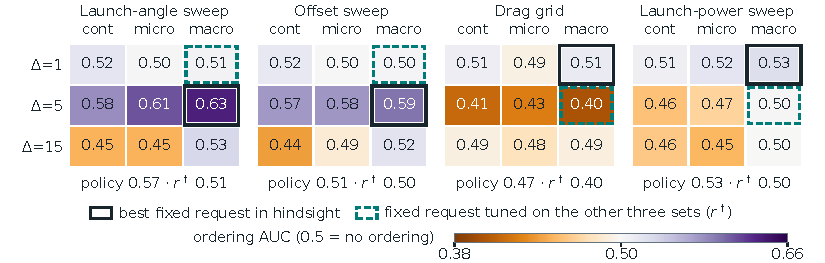
\includegraphics[width=\linewidth]{figures/fig_results_grid.pdf}
\caption{\textbf{The best fixed request changes with the launch set.} Ordering AUC of each of the nine fixed requests on each launch set (hybrid checkpoints, mean over levels and seeds). Solid box: best fixed request in hindsight. Dashed box: the fixed request tuned on the other three sets ($r^\dagger$). Below each panel: the AUC of the request policy and of $r^\dagger$.}
\label{fig:res:grid}
\end{figure}

% ==== BRIEF §6.2 ¶1 (no fixed request suits every set) ================================
% [中] 定位：发现 2：粒度也决定想象结果对候选发射排序得好不好；最佳请求随发射集沿两轴变化；在其他集上调出的固定请求迁移得差。
%      主张：同一关卡内九个固定请求的 AUC 最好与最差平均相差 0.44–0.51（spread：0.497/0.444/0.510/0.491）；(5,macro) 在角度与偏移
%            扫描上第一（0.63、0.59），在拖拽网格上第九（0.40），那里 (1,macro) 最好（0.51）；力度扫描上 (1,macro) 最好（0.53）；
%            最佳请求在四个集上都用 macro，而最佳时距在两个集上为 5、在另两个集上为 1；r† 在任何集上都不是该集的最佳，落后 0.03–0.13
%            （0.635−0.506、0.594−0.504、0.513−0.401、0.527−0.501）。
%      证据：issue-96 comparisons.csv：{inv}_spread、{inv}_auc_F-*；plan.json estimands.cross_fit。
%      手法与边界：不把发射集称为选择方法；不合并集。
% [EN] Role: finding 2: granularity also decides how well imagined outcomes rank candidate launches; the best
%      request varies along both axes; a request tuned elsewhere transfers poorly.
%      Evidence: issue-96 comparisons.csv ({inv}_spread, {inv}_auc_F-*); plan.json cross-fit rule.
%      Craft/Boundaries: launch sets are candidate generators; never pooled.
% ==== /BRIEF ==========================================================================
Granularity also decides how well imagined outcomes rank candidate launches. Within a level, the best and the worst of the nine fixed requests differ by 0.44--0.51 in ordering AUC on average, and which request is best depends on the launch set (Figure~\ref{fig:res:grid}). The request $(5,\textsf{macro})$ ranks first of nine on the angle and offset sweeps (AUC 0.63 and 0.59) but last on the drag grid (0.40), where $(1,\textsf{macro})$ is best (0.51); $(1,\textsf{macro})$ is also best on the power sweep (0.53). The two axes move separately: the best request is $\textsf{macro}$ on every set, while its horizon is 5 on two sets and 1 on the other two. A fixed request tuned on the other three sets therefore transfers poorly. On no set does $r^\dagger$ coincide with the set's best request, and it trails that request by 0.03--0.13.

\subsection{Choosing the request per prediction}
\label{sec:exp:selection}

% ==== BRIEF §6.3 ¶1 (per-prediction choice vs fixed requests) =========================
% [中] 定位：发现 3 前半：逐预测选择请求优于迁移来的固定请求，但未达到事后最佳；并用 Figure 1a 的真实轨迹说明它确实在每次预测时换请求。
%      主张：每个种子的 rollout 中策略在九个请求中的六到七个之间切换；J−r†：角度 +0.060 [0.008, 0.113]、偏移 +0.004 [−0.080, 0.093]、
%            网格 +0.070 [−0.006, 0.144]、力度 +0.027 [−0.069, 0.128]，四个点估计都为正，仅角度区间不含 0；J−事后最佳：−0.069、−0.087、
%            −0.042、+0.001；即在三个集上收回 r† 与事后最佳之间差距的一部分（0.060/0.129、0.004/0.090、0.070/0.112），在力度集上全部收回。
%            Figure 1a 轨迹：发射后单帧步（0–26），交互中 (5,cont)/(5,macro) 交替（26–211），后段 (15,macro)（211–586）。
%      证据：issue-96 comparisons.csv（J-F*、J-F_hindsight）；frequencies.json counts（非零请求数 6、7、6）；issue-92 记录
%            decision.horizon_trace["6"]。
%      手法与边界：区间只作描述；不写"显著"；不写"接触时细"；decision-only。
% [EN] Role: first half of finding 3: per-prediction choice beats the transferred fixed request but not the hindsight
%      best; the real trace in Figure 1a shows the request changing across predictions.
%      Evidence: issue-96 comparisons.csv; frequencies.json (6, 7 and 6 non-zero requests per seed); issue-92 trace.
%      Craft/Boundaries: descriptive intervals; never "fine at contact"; decision-only.
% ==== /BRIEF ==========================================================================
The request policy changes the request from one prediction to the next, using six or seven of the nine requests in each seed's rollouts. Figure~\ref{fig:teaser}(a) shows one such schedule: single-frame steps right after the launch, alternating $(5,\textsf{cont})$ and $(5,\textsf{macro})$ steps through the interaction, and 15-frame $\textsf{macro}$ steps late in the rollout. On the same checkpoints, this per-prediction choice orders launches better than the transferred fixed request $r^\dagger$ on all four sets: by $+0.060$ on the angle sweep, $+0.004$ on the offset sweep, $+0.070$ on the drag grid and $+0.027$ on the power sweep (Figure~\ref{fig:teaser}, b2).

% ==== BRIEF §6.3 ¶2 (compute) =========================================================
% [中] 定位：发现 3 后半：两轴选择以约三分之一的计算量匹配只调时距的自适应基线；节省来自更少的调用（§4：每次调用的代价几乎与 α 无关）。
%      主张：200 个开发状态上遗憾 0.350 对 0.367；每个候选-状态线性 MAC 118.7M 对 356.0M；每状态墙钟 1.0 s 对 2.0 s；
%            每个候选-状态预测器调用 80 对 189。
%      证据：issue-74-matched-dynamics-v1/readiness.json per_seed.*.policies.{hybrid_adaptive, continuous_adaptive}：mean_regret、
%            linear_macs/2400、sum(pair_usage)/2400、mean_perception_planning_seconds 的三种子均值。
%      手法与边界：按 owner 指示保留 "matches"，不补充其他事实；不写训练算力。
% [EN] Role: second half of finding 3: choosing both axes matches the horizon-only adaptive baseline at a third of its
%      compute; the saving comes from fewer calls, since a call costs about the same under every request (Section 4).
%      Evidence: issue-74 readiness.json per-seed policies (three-seed means).
%      Craft/Boundaries: keeps "matches" per owner directive, with no further qualifying facts.
% ==== /BRIEF ==========================================================================
Choosing both axes also saves compute. On the 200 development states, the hybrid's policy matches the horizon-only adaptive baseline, with a regret of 0.350 against 0.367, at a third of its compute: 118.7M against 356.0M multiply-accumulates per candidate and state, and 1.0\,s against 2.0\,s of wall time per state. The saving comes from taking longer steps. The hybrid's policy makes 80 predictor calls per candidate and state where the baseline's makes 189, and a call costs about the same under every request (Section~\ref{sec:mth:model}).

\subsection{How the policy chooses requests}
\label{sec:exp:qual}

% ==== BRIEF FIG (fig:res:qual) ========================================================
% [中] 定位：定性分析主图：运行示例（Figure 1–2 的同一场景，事先选定，非按结果挑选）中，策略为每个候选发射想象时选择的请求序列，
%      以及策略、r†=(1,macro)、事后最佳 (5,macro) 下每个候选按预测代价的排名。
%      证据：figures/build_qualitative_requests.py 读取 issue-96 records（angle, issue-77-n1-001, seed 20260908；J、F-1-macro、
%            F-5-macro）的 decision.schedules 与 ranking，并复用 run_tau_ad_within_checkpoint.load_sources()/build_universe() 的
%            引擎结局连接；a11 为 plan87 typed_dropped_branches，不在冻结候选集中。
%      手法与边界：一个决策、不是频率估计；平局按低序号。
% [EN] Role: the qualitative figure: in the running example (chosen a priori, not by outcome), the request sequence the
%      policy chooses while imagining each launch, and each launch's rank by predicted cost under the policy, r† and
%      the hindsight-best fixed request.
%      Evidence: figures/build_qualitative_requests.py over issue-96 records and the runner's own verdict join.
%      Craft/Boundaries: one decision, not a frequency estimate; ties to the lower ordinal.
% ==== /BRIEF ==========================================================================
\begin{figure}[t]
\centering
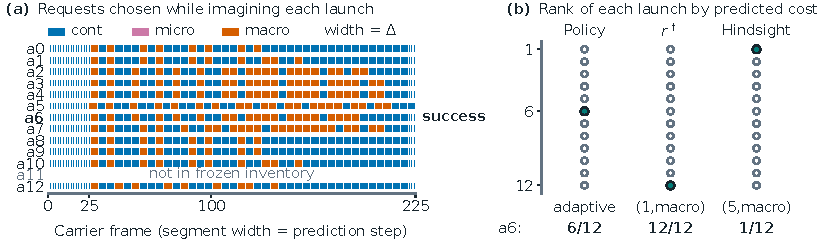
\includegraphics[width=\linewidth]{figures/fig_qualitative_requests.pdf}
\caption{\textbf{One decision, seen through its requests.} The level of Figures~\ref{fig:teaser} and~\ref{fig:levels}, with 12 candidate launches from flat (a0) to steep (a12); only a6 succeeds in the engine. (a) Requests the policy chooses while imagining each launch; each segment is one prediction, coloured by $\alpha$, with width $\Delta$. (b) Rank of each launch by predicted cost (1 = chosen) under the policy, the transferred fixed request $r^\dagger$ and the best fixed request in hindsight; the filled dot is a6. One decision, not a frequency estimate.}
\label{fig:res:qual}
\end{figure}

% ==== BRIEF §6.4 ¶1 (qualitative analysis) ============================================
% [中] 定位：定性分析：策略的请求随想象时间和候选发射而变；在运行示例中其排序介于 r† 与事后最佳之间，与 §6.3 的聚合结果一致；
%      全体 rollout 上的请求构成随时间变化。
%      主张：示例中每个 rollout 都以一次 (1,micro) 和 25 次 (1,cont) 开始，之后交替 (5,cont) 与 (5,macro)，而 macro 步的数量与位置
%            随发射而变（示例中 12 个候选有 8 种不同日程）；a6 在策略下排第 6/12，在 r†=(1,macro) 下第 12/12，在事后最佳 (5,macro)
%            下第 1/12；策略选 a5（失败）。全体 2,634 个 rollout（177 个关卡-种子单元）中，77% 的单元内日程随候选而不同；Δ=5 的份额
%            从前 25 帧的 2% 升到 100 帧之后的 16%，macro 份额从 59% 升到 83%，但单帧步仍占多数（98%、91%、82%）。
%      证据：local 报告 qualitative_requests_report.json（aggregate.bins、differing_schedule_fraction=137/177、example.candidates）；
%            figures/build_qualitative_requests.py。
%      手法与边界：不写"接触时细"；不从一个例子推断频率；如实写单帧步仍占多数。
% [EN] Role: qualitative analysis: the policy's requests change with imagined time and with the launch; in the running
%      example its ranking lies between r† and the hindsight best, as in the aggregate of Section 6.3; across all
%      rollouts the request mix shifts over time.
%      Evidence: qualitative_requests_report.json (aggregate bins; 137/177 differing cells; example candidates).
%      Craft/Boundaries: never "fine at contact"; no frequency from one example; single-frame steps stay the majority.
% ==== /BRIEF ==========================================================================
Figure~\ref{fig:res:qual} opens one decision. While imagining each launch, the policy starts with single-frame steps and then alternates $(5,\textsf{cont})$ and $(5,\textsf{macro})$, and where it places the $\textsf{macro}$ steps depends on the launch: the 12 candidates receive eight different schedules. The resulting order sits between the two fixed references, as in the aggregate. The policy ranks the one successful launch, a6, sixth of 12, the transferred fixed request $(1,\textsf{macro})$ ranks it last, and the best fixed request in hindsight, $(5,\textsf{macro})$, ranks it first. The same behaviour holds across all 2,634 imagined rollouts. In 77\% of level--seed pairs the schedule differs between candidate launches, so the choice depends on the imagined state and not only on the time step. Longer and coarser requests become more frequent as the rollout proceeds: the share of $\Delta=5$ rises from 2\% of predictions in the first 25 frames to 16\% after frame 100, and the share of $\textsf{macro}$ from 59\% to 83\%.
